\documentclass[12pt, letterpaper, fleqn]{article}
\usepackage[letterpaper, margin=.75in]{geometry}
\usepackage[utf8]{inputenc}
\usepackage{amsmath}
\usepackage{amssymb}
\usepackage{algorithmicx}
\usepackage{algpseudocode}
\usepackage{algorithm}
\usepackage[english]{babel}
\usepackage{amsthm}
\usepackage{graphicx}
\usepackage{xcolor}
\graphicspath{ {.} }
\usepackage{fancyhdr}
\usepackage{tikz}
\usepackage{hyperref}
\usepackage{cancel}
\newcommand*\circled[1]{\tikz[baseline=(char.base)]{
            \node[shape=circle,draw,inner sep=2pt] (char) {#1};}}
\setlength\parindent{0pt}
\def\fullouterjoin{\mathbin{\ojoin\mkern0mu\bowtie\mkern3mu\ojoin}}

%\pagestyle{fancy}
%\fancyhf{}
%\rhead{Bill Yang}
%\renewcommand{\headrulewidth}{0pt}

\newcommand{\handout}[5]{
   \renewcommand{\thepage}{#1-\arabic{page}}
   \noindent
   \begin{center}
   \framebox{
      \vbox{
%    \hbox to 5.78in { {\bf M328K Number Theory} \hfill #2 }
%       \vspace{4mm}
%       \hbox to 5.78in { {\Large \hfill #5  \hfill} }
%       \vspace{2mm}
%       \hbox to 5.78in { {\it #3 \hfill #4} }
    \hbox to 5.78in { { Bill Yang} \hfill {Due: #2} }
       \vspace{4mm}
       \hbox to 5.78in { {\Large \hfill #5  \hfill} }
       \vspace{2mm}
       \hbox to 5.78in { {#3 \hfill #4} }
      }
   }
   \end{center}
   \vspace*{4mm}
}

\newcommand{\ho}[5]{\handout{#1}{#2}{#3}{Instructor: #4}{Homework #1}}

\begin{document}
  \ho{7}{3/30/20}{CS386D Database Systems}{Daniel Miranker} \\

  \section{Part A}

  \textbf{15.3.2} \\
  $B(S) + (B(S)B(R)) / (M - 1) = 10000 + \lceil (10000/(1000-1)\rceil \times 10000) = \\
  120000$ disk I/O. \\
  
  \textbf{15.3.3 a} \\
  \begin{align*}
    100000 &= 10000 + \lceil 10000/ (M-1)\rceil (10000)  \\
    M &= 1112.11
  \end{align*}
  $M \geq 1113$ \\

  \textbf{15.4.2 a, b, c} \\
  a) $3( B(S) + B(R) ) = 3 ( 10000 + 10000) = 60000$ I/Os. \\
  b) $5( B(S) + B(R)) = 5 ( 10000 + 10000 ) = 100000$ I/Os.\\
  c) $3( B(S) + B(R) ) = 3 ( 10000 + 10000) = 60000$ I/Os. \\
  

  \textbf{15.4.3} \\
  For 2PPMS, we can decrease the size of the sublists such that we do have M
  sublists, eg.  we only use $pM$ buffers to sort sublists and sublists are $pM$
  long where $0 <p < 1$. Then when we sort a sublist, we can place the first
  block of the sublist in our unused blocks, the $(1-p)M$ blocks not used for
  sorting, until these are full. Then the algorithm would be more or less the
  same, where we must write out entire lists and reread them to merge sort. Thus
  we save $2 ((1-p)M)$ disk I/Os.


  \section{Part B}

  \textbf{16.4.1 a, d, i} \\
  a) \\
  $\frac{100 \times 200 \times 300 \times 400} {60 \times 100 \times 50} = 
  8000$ tuples     \\\\
  d) Selection gives us $T(\sigma_{c=20}(Y)) = 6$.\\
  $\frac{6 \times 400}{50} = 48$ tuples.  \\\\
  i) $\frac{200 \times 300 }{3} = 20000$ tuples. \\

  \section{Part C}
  1. Text problem 16.6.1a, (which concerns precisely part a of 16.4.1). In
  addition to answering the text question, show the entries in the dynamic
  programming matrix. \\
  
  \begin{center}
  \begin{tabular} {| c | c | c | c |}
  \hline
  W & X & Y & Z\\
  \hline
  \end{tabular} \\
  \begin{tabular} { c | c | c | c | c }
  & W & X & Y & Z \\
  \hline
  Size & 100  & 200  & 300 & 400\\
  Cost & 0    & 0    & 0   & 0 \\
  Best Plan & W & X & Y & Z \\
  \end{tabular}
  \end{center}
  

  \begin{center}
  \begin{tabular} {| c | c | c | c | c | c |}
  \hline
  WX & WY & WZ & XY & XZ & YZ \\
  \hline
  W & X & Y & Z & & \\
  \hline
  \end{tabular} \\
  \begin{tabular} { c | c | c | c | c | c | c }
  & (W, X) & (W, Y) & (W, Z) & (X, Y) & (X, Z) & (Y, Z) \\
  \hline
  Size & 333 & 30000 & 40000 & 600 & 80000 & 2400 \\
  Cost & 0 & 0 & 0 & 0 & 0 & 0\\
  Best Plan & W \fullouterjoin X & W \fullouterjoin Y & W \fullouterjoin Z & X
  \fullouterjoin Y & X \fullouterjoin Z & Y \fullouterjoin Z \\
  \end{tabular}
  \end{center}

  \begin{center}
  \begin{tabular} {| c | c | c | c | c | c |}
  \hline
  WXY & WXZ & WYZ & XYZ & &\\
  \hline
  WX & WY & WZ & XY & XZ & YZ \\
  \hline
  W & X & Y & Z & & \\
  \hline
  \end{tabular}\\
  \begin{tabular} { c | c | c | c | c }
  & (W, X, Y) & (W, X, Z) & (W, Y, Z) & (X, Y, Z)  \\
  \hline
  Size & 1000 & 133333 & 240000 & 4800 \\
  Cost & 333  & 333 & 2400 & 600  \\
  Best Plan & Y \fullouterjoin (W \fullouterjoin X)  & (W \fullouterjoin X)
  \fullouterjoin Z & W \fullouterjoin (Y \fullouterjoin Z) & Z \fullouterjoin (X \fullouterjoin Y)
  \\
  \end{tabular}
  \end{center}

  \begin{center}
  \begin{tabular} {| c | c | c | c | c | c |}
  \hline
  WXYZ & & & & & \\
  \hline
  WXY & WXZ & WYZ & XYZ  & &  \\
  \hline
  WX & WY & WZ & XY & XZ & YZ \\
  \hline
  W & X & Y & Z & & \\
  \hline
  \end{tabular}\\
  \begin{tabular} { c | c  }
  Plan & Cost \\ 
  \hline
  Z \fullouterjoin (Y \fullouterjoin (W \fullouterjoin X)) &  1333 \\
  Y \fullouterjoin ((W \fullouterjoin X) \fullouterjoin Z )&  133666\\
  X \fullouterjoin (W \fullouterjoin (Y \fullouterjoin Z)) & 242400 \\
  W \fullouterjoin (Z \fullouterjoin (X \fullouterjoin Y)) &  5400 \\
  (W\fullouterjoin X) \fullouterjoin (Y \fullouterjoin Z)  & 2733 \\
  (W \fullouterjoin Y) \fullouterjoin (X \fullouterjoin Z) & 110000 \\
  (X \fullouterjoin Y) \fullouterjoin (W \fullouterjoin Z) & 40600 \\


  \end{tabular}
  \end{center}\\
  $Z \fullouterjoin (Y \fullouterjoin (W \fullouterjoin X))$ is the best plan
  \\\\


  2. Repeat 16.6.1a, this time.  \\
  a) draw the query graph.   \\
  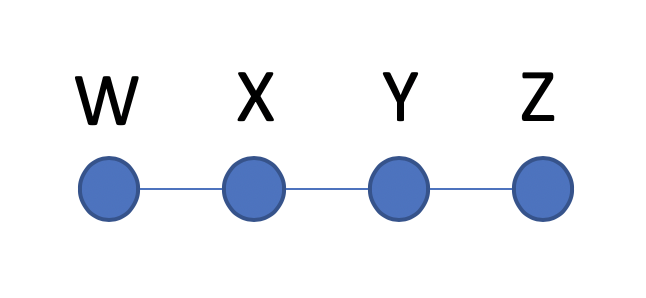
\includegraphics[scale=0.5]{query_graph.png}


  b) leveraging the 
  query graph to avoid Cartesian products, limit the amount of work and number
  of entries you create in the dynamic programming matrix. \\

\begin{center}
  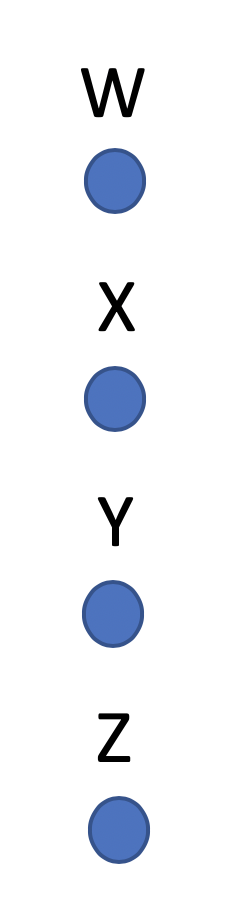
\includegraphics[scale=0.25]{1_relation.png}
  \begin{tabular} {| c | c | c | c |}
  \hline
  W & X & Y & Z\\
  \hline
  \end{tabular}\\
  \begin{tabular} { c | c | c | c | c }
  & W & X & Y & Z \\
  \hline
  Size & 100  & 200  & 300 & 400\\
  Cost & 0    & 0    & 0   & 0 \\
  Best Plan & W & X & Y & Z \\
  \end{tabular}
\end{center}

\begin{center}
  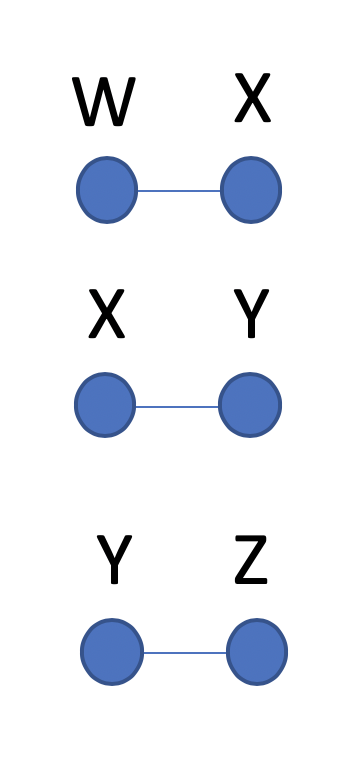
\includegraphics[scale=0.25]{2_relation.png}
  \begin{tabular} {| c | c | c | c | c | c |}
  \hline
  WX & \cancel{WY} & \cancel{WZ} & XY & \cancel{XZ} & YZ \\
  \hline
  W & X & Y & Z & & \\
  \hline
  \end{tabular} \\
  \begin{tabular} { c | c | c | c  }
  & (W, X) & (X, Y) & (Y, Z) \\
  \hline
  Size & 333 &  600 & 2400 \\
  Cost & 0 & 0 & 0 \\
  Best Plan & W \fullouterjoin X & X \fullouterjoin Y & Y \fullouterjoin Z \\
  \end{tabular}
\end{center}

\begin{center}
  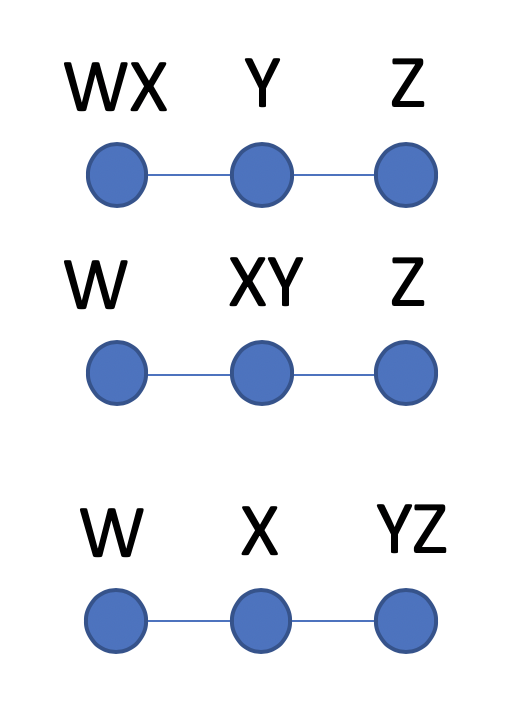
\includegraphics[scale=0.25]{3_relation.png}
  \begin{tabular} {| c | c | c | c | c | c |}
  \hline
  WXY & \cancel{WXZ} & \cancel{WYZ} & XYZ & &  \\
  \hline
  WX & \cancel{WY} & \cancel{WZ} & XY & \cancel{XZ} & YZ \\
  \hline
  W & X & Y & Z & & \\
  \hline
  \end{tabular}\\
  \begin{tabular} { c | c | c  }
  & (W, X, Y) & (X, Y, Z)  \\
  \hline
  Size & 1000 & 4800 \\
  Cost & 333  & 600  \\
  Best Plan & Y \fullouterjoin (W \fullouterjoin X)  & Z \fullouterjoin (X \fullouterjoin Y)
  \\
  \end{tabular}
\end{center}

\begin{center}
  \begin{tabular} {| c | c | c | c | c | c |}
  \hline
  WXYZ & & & & & \\
  \hline
  WXY & \cancel{WXZ} & \cancel{WYZ} & XYZ & &  \\
  \hline
  WX & \cancel{WY} & \cancel{WZ} & XY & \cancel{XZ} & YZ \\
  \hline
  W & X & Y & Z & & \\
  \hline
  \end{tabular}
  \begin{tabular} { c | c  }
  Plan & Cost \\ 
  \hline
  Z \fullouterjoin (Y \fullouterjoin (W \fullouterjoin X)) &  1333 \\
  W \fullouterjoin (Z \fullouterjoin (X \fullouterjoin Y)) &  5400 \\
  (W\fullouterjoin X) \fullouterjoin (Y \fullouterjoin Z) & 2733 \\
  \end{tabular}
\end{center}

\end{document}
